\documentclass[12pt]{article}
\usepackage[utf8]{inputenc}
\usepackage{authblk} %autores
\usepackage{bm}% bold math
\usepackage{amsmath} %mates
\usepackage{amssymb} %mates
\usepackage{stmaryrd}

\usepackage[spanish]{babel} %Idioma

%\usepackage{natbib} %Bibliografía
\usepackage[backend=biber]{biblatex}
\bibliography{referencias}

\usepackage{geometry,pdfpages} %Márgenes
\usepackage{enumerate}
\usepackage{vmargin}

\usepackage{setspace}

\usepackage{graphicx} %gráficos
\graphicspath{ {./tables/}} %Camino de gráficos

\usepackage{tabularx} %Config. tablas

\usepackage{fancyhdr}  %más márgenes y encabezado
\usepackage{blindtext}
\usepackage{parskip}

\renewcommand{\thesection}{\Roman{section}}

\usepackage[font=small,labelfont=bf]{caption}

\setpapersize{A4}
\setmargins{2.5 cm}       % izquierdo
{1.5 cm}                  % superior
{16 cm}                   % ancho texto
{25.5 cm}                 % altura texto
{5 pt}                    % altura encabezados
{0.5 cm}                  % espacio texto - encabezados
{100 pt}                  % alto pie de página
{0cm}                     % espacio texto y - pie de página


\title{\textbf{\large{Análisis de la cantidad de Monóxido de Carbono en la zona Noroeste de la Ciudad de México}}} 
\author{\normalsize Norma Angélica Márquez Sulca\\ 427278 \\\normalsize Universidad de Guanajuato - División de Ciencias e Ingenierías UG-CL\vspace{-1em}} 

\date{\small{17 de junio de 2020}\vspace{1em}}


\begin{document} %inicio del documento 

    \maketitle %imprimir título, autores y affil 
        
      \begin{abstract} 
        Con datos obtenidos respecto a la calidad del aire en las distintas zonas de Ciudad de México, se determinó un área y gas específico a estudiar. Se predijó la cantidad del mismo en la zona seleccionada para años posteriores.
      \end{abstract}

\setlength{\topmargin}{0mm} %Eleva el margen del título

\section{\centering{\small{INTRODUCCIÓN}}}
    Dentro de la página del Gobierno de la ciudad de México \cite{CDMX} se descargaron datos de “Índice de calidad del aire”, fueron utilizados los de 2010 hasta 2018, se emplearon únicamente los datos del noroeste de la ciudad de México y del gas Monóxido de carbono y se desea predecir la contaminación con base en estos parámetros para 2019, 2020, 2021.
 
\section{\centering{\small{DESARROLLO}}}
    El análisis se realizó en Python, por lo que, lo primero que se hizo fue importar las librerías necesarias para la manipulación de los datos.
         \begin{figure}[h] 
          \centering 
            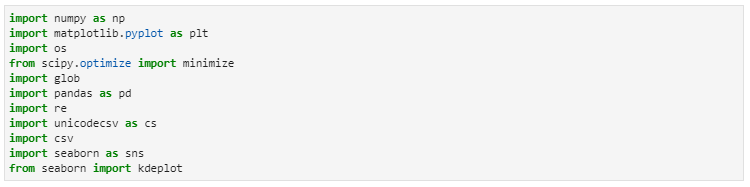
\includegraphics[width=12cm]{Pred1.png}
                \caption{Importando las librerías.}
                \label{fig:1}
                 \end{figure}  
    
    Después de esto, se cargaron los archivos necesarios para realizar la predicción, en total son 9 archivos, contenidos en una carpeta nombrada "DatosHIGI2", uno por cada año a estudiar, y se creó una variable que los almacenara a todos.          
         \begin{figure}[h] 
          \centering 
            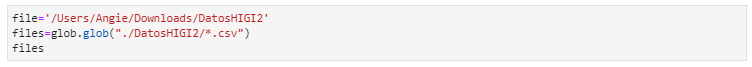
\includegraphics[width=12cm]{Pred2.png}
                \caption{Ruta de los archivos.}
                \label{fig:2}
                 \end{figure}  
        
    Para estudiar el comportamiento de los datos, se filtraron únicamente las columnas $"$Fecha$"$ y "Noroeste monóxido de carbono" de los archivos , dado que estas son las únicas que serán de nuestro interés, inmediatamente después del filtro, se uso la función "pd.to\_datetime()", para que reconociera las fechas escritas en la columna de fechas y nos permitiese agruparlo en el intervalo necesario, ya que se nos proporcionaba la información por horas, por lo que cada día del año se repetía 24 veces. 
         \begin{figure}[h] 
          \centering 
            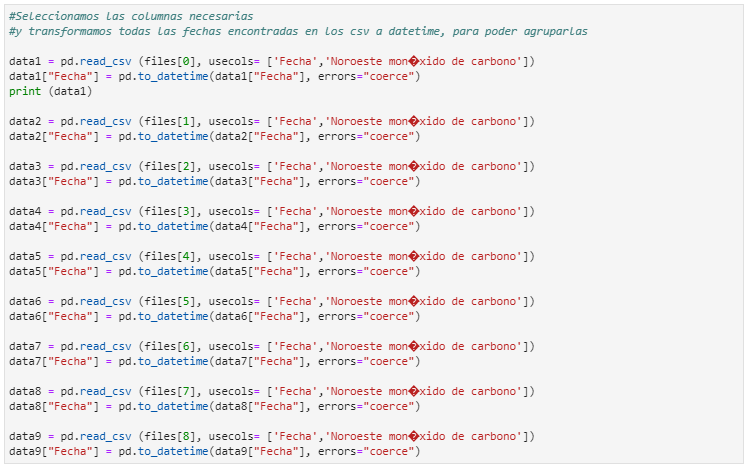
\includegraphics[width=12cm]{Pred3.png}
                \caption{Lectura y filtro de los archivos.}
                \label{fig:3}
                 \end{figure}  
    
    Durante la elaboración de tablas, se presentó un sorting, causando que la agrupación de datos fuese incorrecta, ya que comenzaba brindando los días primero de cada mes, después los segundos y progresivamente, por tanto, si se deseaba obtener la suma de un mes en específico, esta resultaba incorrecta, para resolver este error se utlizó la función \"groupby\" con "sort=Flase". 
        \begin{figure}[h!] 
          \centering 
            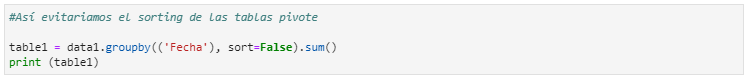
\includegraphics[width=12cm]{Pred4.png}
                \caption{Código para evitar sorting en las tablas.}
                \label{fig:4}
                 \end{figure} 
                 
         \begin{figure}[h!] 
          \centering 
            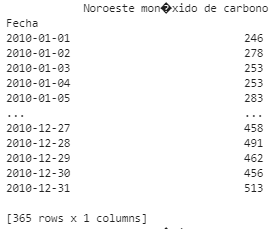
\includegraphics[width=7cm]{Pred4_1.png}
                \caption{Tablas con sorting.}
                \label{fig:5}
                 \end{figure} 
            
         \begin{figure}[h!] 
          \centering 
            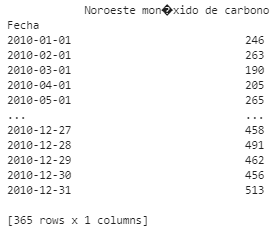
\includegraphics[width=7cm]{Pred4_2.png}
                \caption{Tablas sin sorting.}
                \label{fig:6}
                 \end{figure} 
             
    Se decidió agrupar por año los valores, de esta manera, el sorting dejó de ser relevante. Esto se realizó a través de tablas pivote con la función "pd.pivot\_table\" y el comando: freq=$"$y$"$. 
         \begin{figure}[h!] 
          \centering 
            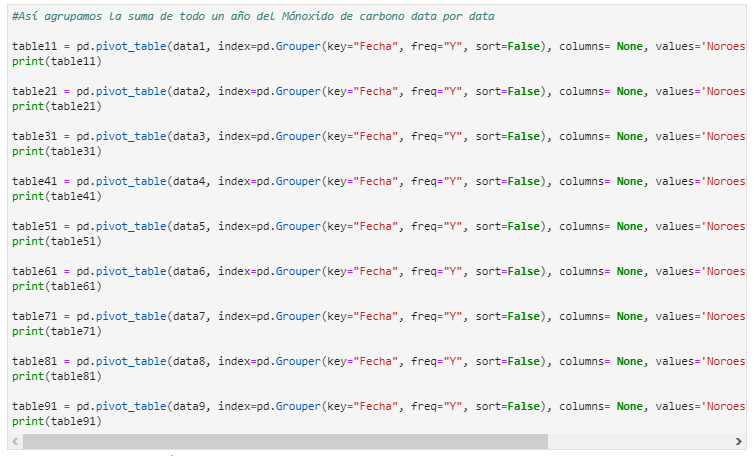
\includegraphics[width=11cm]{Pred5.png}
                \caption{Tablas pivote que regresan la suma anual de Mónoxido.}
                \label{fig:7}
                 \end{figure}      
     
    Se elaboró un ciclo que te le asignará a cada año, su archivo correspondiente. Primero, se agruparon los valores de cada fecha, en este caso de cada año, y se acomodaron cronológicamente, posteriormente, se le destino a cada una el archivo que coincidera con la fecha. Además se creó un arreglo que contiene cada uno de lo años utilizados. 
         \begin{figure}[h!] 
          \centering 
            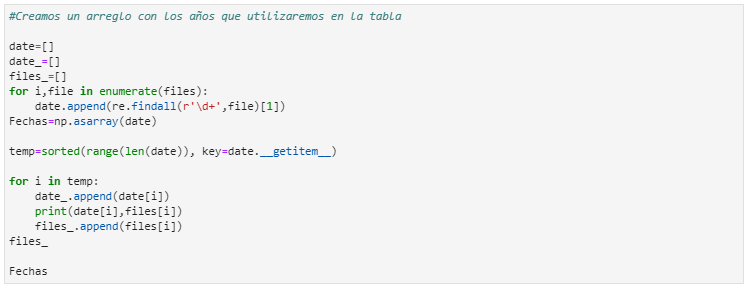
\includegraphics[width=11cm]{Pred6.png}
                \caption{Ciclo para elaborar el arreglo de Fechas.}
                \label{fig:8}
                 \end{figure}  
     
    Se estructuró otro ciclo, que imprimera cada uno de los años y su suma correspondiente de Mónoxido de carbono, a su vez se guardó en un arregló llamado "arreglo\_info" cada uno de los pares de datos que generó el ciclo recién mencionado.
        \begin{figure}[h!] 
          \centering 
            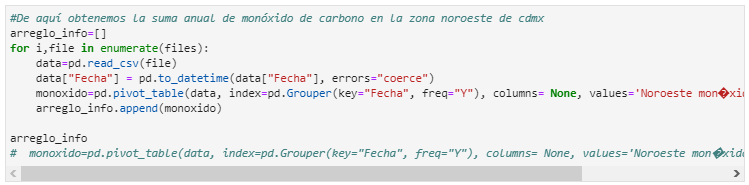
\includegraphics[width=12cm]{Pred7.png}
                \caption{Ciclo que imprime las tablas pivote de la figura[\ref{fig:7}]}
                \label{fig:9}
                 \end{figure}  
    
    Para facilitar el manejo de la información, se creó un arreglo con la suma del Monóxido de carbono de cada año. 
         \begin{figure}[h!] 
          \centering 
            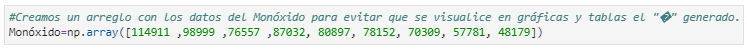
\includegraphics[width=12cm]{Pred8.png}
                \caption{Arreglo de las sumas de Monóxido.}
                \label{fig:10}
                 \end{figure}  
    
    Se creó un DataFrame llamado "tabla\_t"que contuviese únicamente dos columnas, utilizando los arreglos "Fechas\" y "Monóxido". 
         \begin{figure}[h!] 
          \centering 
            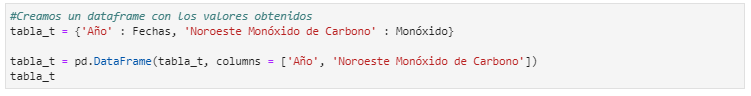
\includegraphics[width=12cm]{Pred9.png}
                \caption{DataFame agrupado por Fechas y Monóxido.}
                \label{fig:11}
                 \end{figure}
    
    Utilizando Matplotlib, graficamos ambos arreglos, colocando los años en el eje x, y la cantidad de Monóxido de carbono en el eje y, 
         \begin{figure}[h!] 
          \centering 
            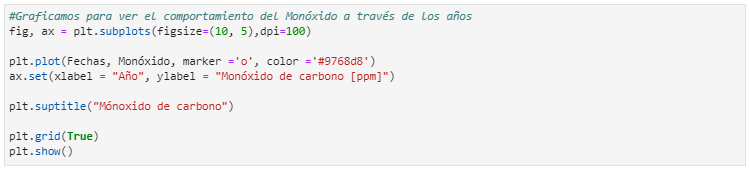
\includegraphics[width=12 cm]{Pred10.png}
                \caption{Código para la gráfica de los datos del DataFrame.}
                \label{fig:12}
                 \end{figure}  
             
    
    Al observar la gráfica y  su comportamiento, se decidió hacer un ajuste lineal para elaborar nuestra predicción.Con la función "polyfit" se realizó la regresión lineal y se almacenaron los valores de la pendiente y ordenada al origen. 
         \begin{figure}[h!] 
          \centering 
            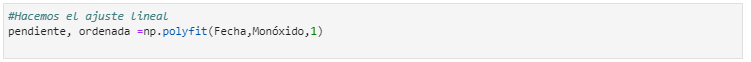
\includegraphics[width=12cm]{Pred12.png}
                \caption{Ajuste lineal.}
                \label{fig:13}
                 \end{figure}  
                       \begin{figure}[h] 
          \centering 
            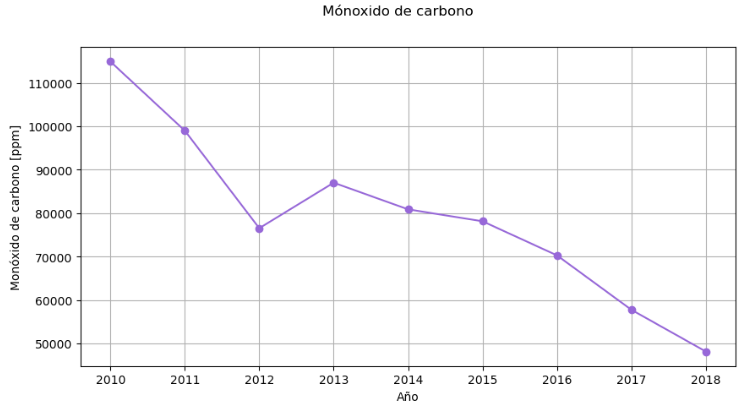
\includegraphics[width=12cm]{Pred11.png}
                \caption{Grafica de los datos antes del ajuste lineal.}
                \label{fig:14}
                 \end{figure}  
             

    Conociendo la ecuación de una recta donde y=mx+b, se sustituyeron los valores de "m" y "b" obtenidos del código anterior, guardados en "pendiente" y "ordenada" y asignado a "x" los valores: 10, 11 y 12, correspondientes a los años 2019, 20201 y 2021, respectivamente; para de esta manera ser capaces de cálcular nuestra predicción.
         \begin{figure}[h] 
          \centering 
            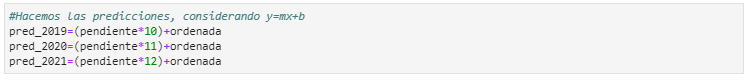
\includegraphics[width=12cm]{Pred13.png}
                \caption{Predicción.}
                \label{fig:15}
                 \end{figure}  

 \section{\centering{\small{CONCLUSIÓN}}}
 Para 2019 se predijo un total de 44 872.05555555553 ppm de Mónoxido de carbono en la zona Noroeste de la Ciudad de Mexico; para 2020, 38006.08888888886 ppm y para 2021, 31140.1222222222 ppm, redondeando los datos, obtendriamos la siguiente tabla como resultado, podemos observar que verdaderamete se ha reducido su cantidad en el aire con el transcurrir de los años y se espera que siga disminuyendo.
 \begin{table*}[h!]
  \centering
        \begin{tabular}{ |p{3cm}|p{3cm}|}
         \hline
         Año & Monóxido de carbono [ppm]\\ 
         \hline
         2019  & 44 872\\
         \hline 
         2020  & 38 006 \\
          \hline
         2021  &  31 140 \\
          \hline
         \end{tabular}
               \vspace{1em}
         \caption{Tabla de resultados.}
        \label{tab:1}
    \end{table*}
 
 \newpage
 \begin{center}
\begin{spacing}{2} % factior = 2
\textbf{\large Análisis de número de casillas de votación electoral a instalar en el estado de Guanjauato}
 \end{spacing}
 \end{center}

 
  \begin{abstract} 
  Se analizaron los datos de la Estadística de Padrón Electoral y Lista Nominal de Electores de Guanajuato con los datos proporcionados por el INE, para, filtrando y manipulando adecuadamente los datos, ser capaces de predecir la cantidad de actas y de casillas que serán necesarias para febrero 2021.
  \end{abstract}


\setlength{\topmargin}{0mm}

 \section{\centering{\small{INTRODUCCIÓN}}}
 Dentro de la página del Instituto Nacional Electoral \cite{INE} se descargaron datos de “Estadística de Padrón Electoral y Lista Nominal de Electores”, fueron utilizados los de la lista nominal desde septiembre de 2019 hasta diciembre de 2020, se utilizaron únicamente los datos del estado de Guanajuato (estado=11) y se desea predecir los de febrero de  a través de un ajuste lineal.
 
  \section{\centering{\small{DESARROLLO}}}
 Este análisis se realizó en Phyton, por lo que lo primero que se realizó fue importar las librerías que se usarían para el mismo, considerando las necesidades de filtrar tablas, realizar cálculos entre columnas, crear arreglos, entre otros.
  \begin{figure}[h] 
  \centering 
    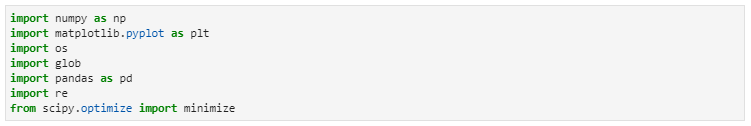
\includegraphics[width=12cm]{Imagen1.png}
        \caption{Importando las librerías.}
        \label{fig:16}
        \end{figure}  
        
Después de esto, se cargaron los archivos necesarios para realizar la predicción y se creó una variable que los almacenara a todos. Fueron 16 archivos en total nombrados al principio por el mes, textualmente, y después, por su año y mes, númericamente, por ejemplo: Septiembre\_201909.
  \begin{figure}[h] 
  \centering 
    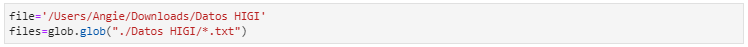
\includegraphics[width=12cm]{Imagen2.png}
        \caption{Carga de los archivos ".txt".}
        \label{fig:17}
        \end{figure} 
         
A continuación, se eligió uno de los archivos, del que se seleccionaron únicamente 5 columnas: "ENTIDAD", "DISTRITO", "MUNICIPIO", "SECCION Y "LISTA\_NAL", en "data1"; este también se filtró por entidad, en "data\_gto", eligiendo únicamente la 11, correspondiente a Guanajauto. Esto fue realizado para analizar el orden y comportamiento de los datos de maneras más simple y clara. 

  \begin{figure}[h] 
  \centering 
    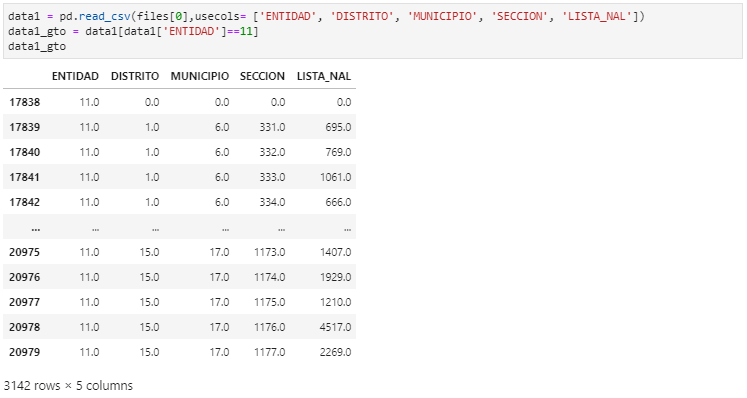
\includegraphics[width=12cm]{Imagen3.png}
        \caption{Creación de la primer tabla.}
        \label{fig:18}
         \end{figure}  

Se elaboró un ciclo que te le asignará a cada año, su archivo correspondiente. Primero, se agruparon los valores de cada fecha, en este caso de cada año, y se acomodaron cronológicamente, posteriormente, se le destino a cada una el archivo que coincidera con la fecha.

    \begin{figure}[h] 
    \centering 
    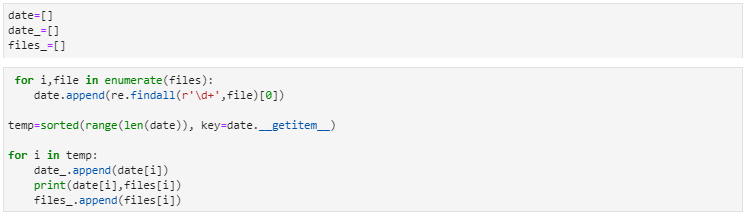
\includegraphics[width=12cm]{Imagen4.png}
        \caption{Ciclo de las fechas existentes en los archivos.}
        \label{fig:19}
         \end{figure}     

El siguiente paso  fue graficar los datos para obeservar su comportamiento y comprobar que siguiese una tendencia lineal para poder aplicar una regresión lineal y ser capaces de realizar nuestra predicción. Como podemos observar en la fig[\ref{fig:20}].

       \begin{figure}[h!] 
       \centering 
    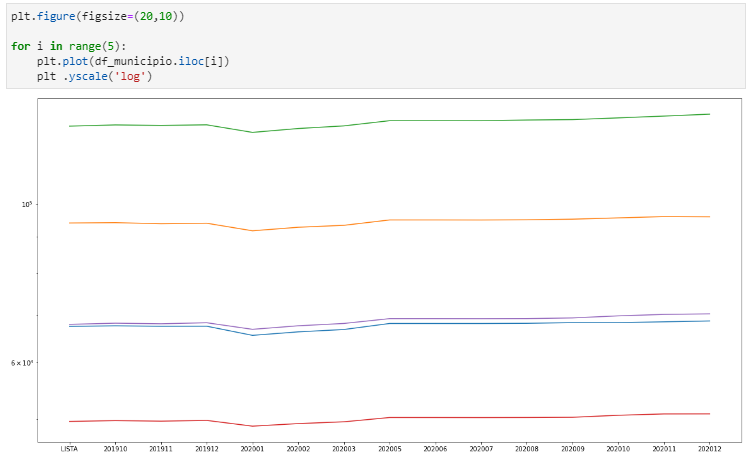
\includegraphics[width=9cm]{Imagen5.png}
        \caption{Grafica de 5 municipios.}
        \label{fig:20}
         \end{figure}

Convertimos nuestro DataFrame en un arreglo, de está manera podremos utilizarlo fácilmente en la función de la regresión. Volvemos a graficar para asegurarnos de que no hemos modificado los valores. 

       \begin{figure}[h] 
       \centering 
    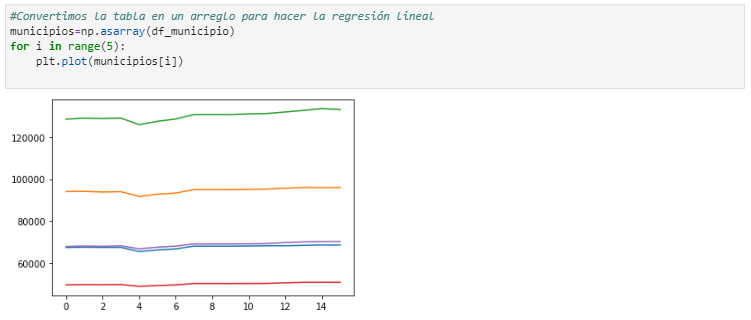
\includegraphics[width=12cm]{Imagen6.png}
        \caption{Conviertiendo nuestra tabla en un arreglo.}
        \label{fig:21}
         \end{figure} 
         

Posteriormente, elaboramos un arreglo que genere la regresión lineal por cada municipio y guardamos los valores que nos arroja de la pendiente y ordenada al origen en "na$"$ y "ba", reespectivamente;  los aplicamos, utilizando la fórmúla y=mx+b y guardamos los datos en la variable "predicción\_lineal".
       \begin{figure}[h] 
       \centering 
    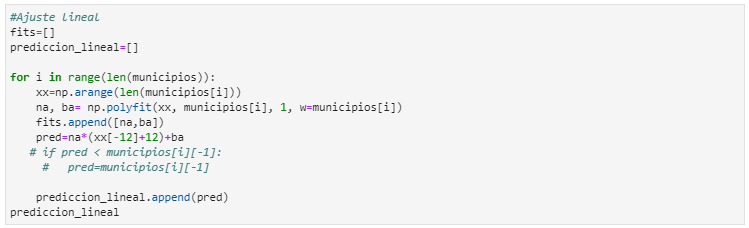
\includegraphics[width=12cm]{Imagen7.png}
        \caption{Regresión lineal por municipio.}
        \label{fig:22}
         \end{figure} 

Añadimos la columna de predicción a la tabla que ya habíamos filtrado anteriormente por municipio.
       \begin{figure}[h] 
       \centering 
    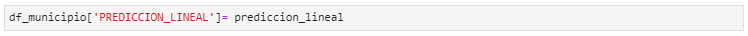
\includegraphics[width=12cm]{Imagen8.png}
        \caption{Añadimos la predicción al DataFrame}
        \label{fig:23}
         \end{figure} 
         
Realizamos una suma con todos los valores dados por la predicción, para obtener la cantidad de actas nececarias.
       \begin{figure}[h!] 
       \centering 
    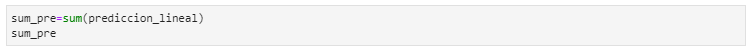
\includegraphics[width=12cm]{Imagen9.png}
        \caption{Suma de las predicciones.}
        \label{fig:24}
         \end{figure} 
         
Finalmente, divimos entre 750, ya que se consideran 750 actas por cada casillas
       \begin{figure}[h!] 
       \centering 
    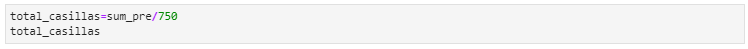
\includegraphics[width=12cm]{Imagen10.png}
        \caption{División para obtener el número de actas.}
        \label{fig:25}
         \end{figure} 

\section{\centering{\small{CONCLUSIÓN}}}
Se obtuvo un total de 6042.567323217931 actas, ya de que debemos reportar un número entero, resultaría en 6043 actas necesarias para febrero 2021. También se intentó estimar esta misma cantidad aplicando el ajuste por secciones, lo que nos daría un resultado de 7688 casillas, valor obtenido en el mismo proyecto cuando fue elaborado en Excel, sin embargo, no fui capaz de crear un código que nos brindará tal resultado.  
\vspace{2em}
  
\printbibliography

    
\end{document}
